%%%%%%%%%%%%%%%%%%%%%%%%%%%%%%%%%%%%%%%%%%%%%%%%%%%%%%%%%%%%%%%%%%%%%%%%%%%%%%%%
%2345678901234567890123456789012345678901234567890123456789012345678901234567890
%        1         2         3         4         5         6         7         8

\documentclass[letterpaper, 10 pt, conference]{ieeeconf}
\IEEEoverridecommandlockouts
\overrideIEEEmargins
\usepackage{cite}
\usepackage{amsmath,amssymb,amsfonts,amsthm,color,float}
\usepackage{algorithmic}
\usepackage{graphicx}
\usepackage{textcomp}
 \usepackage{calc}
 \usepackage{tikz}
\usepackage{cases}
\usepackage{verbatim}
\usepackage{hyperref}
\usepackage{xcolor, soul}
\usepackage{mathtools, nccmath}

\theoremstyle{plain}
\newtheorem{thm}{Theorem}
\newtheorem{cor}{Corollary}
\newtheorem{prop}{Proposition}
\newtheorem{conj}{Conjecture}
\newtheorem{lemma}{Lemma}
\newtheorem{claim}{Claim}

\theoremstyle{definition}
\newtheorem{defn}{Definition}
\newtheorem{assum}{Assumption}
\newtheorem{ex}{Example}
\newtheorem*{rem*}{Remark}

\theoremstyle{remark}
\newtheorem{obs}{Observation}


% general math notation
\renewcommand{\rm}[1]{\mathrm{#1}}
\newcommand{\bb}[1]{\mathbb{#1}}
\newcommand{\cl}[1]{\mathcal{#1}}
\newcommand{\R}{\bb{R}}
\newcommand{\N}{\bb{N}}



\begin{document}
\title{Designing Efficient Algorithms in Resource Utilization with Degradation}
\author{Bryce L. Ferguson and Rohit Konda}

\maketitle
\thispagestyle{empty}

The main thesis of this research proposal is on the design and analysis of adaptive algorithms that dictate the utilization of resources whose quality may be dynamic. A distinct feature of this setting is that as a resource is utilized, its current operating quality degrades. As such, effective algorithms must manage the short-term long-term trade-off. 

Providing good algorithms in this framework has deep implications in various application domains. For example, consider ride-sharing platforms; these services have become ubiquitous, and so operating these platforms in an efficient manner is vital for rider satisfaction and minimizing usage costs. 
Ride-sharing platforms inherit this trade-off from the following perspective. Drivers span through areas of an urban landscape depending on the present rider demand. Rider demand (modeled as a resource of un-serviced riders) in areas that are serviced by drivers are expected to decrease while areas that are not serviced are expected to accumulate a surplus of rider demand. As such, desirable routing mechanisms for drivers should adaptively allocate drivers in response to the dynamic current rider demand, while also managing possible future demand. Managing this fundamental trade-off of resource utilization appears in various other application domains as well, including battery power storage/utilization, server queuing, task-assignment, renewable energy sources, and more.

With this in mind, we propose to study a general dynamic resource utilization problem where a resource's quality degrades as a function of its utilization. We take inspiration from \emph{fishery games} that were studied in the economics literature in the 1980's, where the emphasis  was on protecting a common resource from over-utilization. However, in our work, we focus on questions on resource-utilization from a novel engineering perspective. This new perspective offers new opportunities for applying relevant tools but also new challenges presented by the engineering problem domains.

More formally, the resource utilization problem is characterized by a set of agents that can decide to utilize a certain portion of resources at each point in time; the agents, as a whole, generate value or benefit from their use of the selected resources. However, the utilization of a resource can affect its quality or availability in the future (e.g., farming fish from a lake today means less fish in that lake tomorrow). In this sense, greedy utilization in the short term by agents can lead to deficiencies in the long-term. To the agents, there exists a natural trade-off, in which they must balance short and long-term gains when utilizing resources. This trade-off is precisely what we seek to analyze. In this pursuit, several important and interesting questions emerge:
\\

\begin{figure}
    \centering
    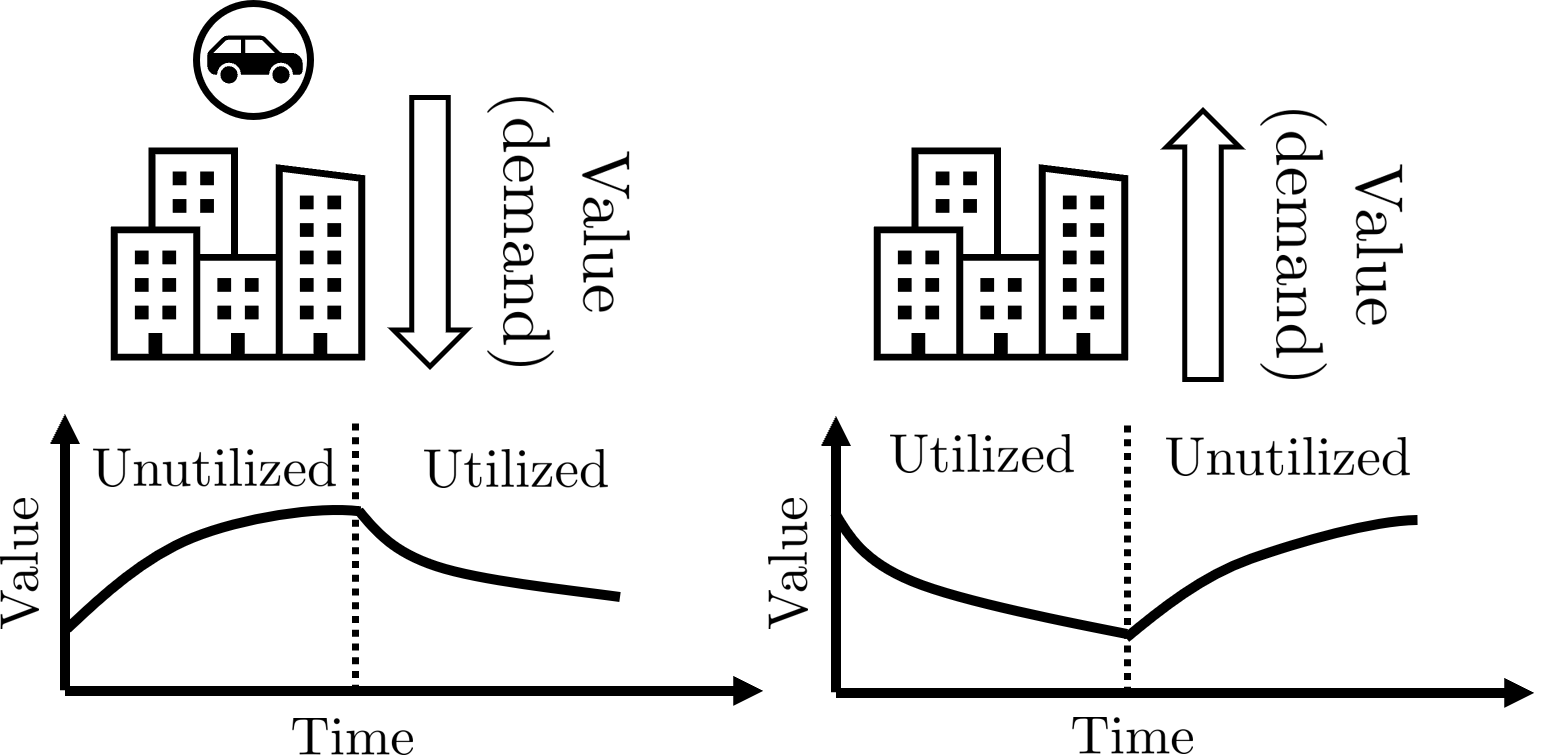
\includegraphics[width=\columnwidth]{fig_city_2.png}
    \caption{An illustration of a neighborhood (resource) being serviced (utilized) by urban transit vehicles (agents). While an area is being serviced, the demand (or quality) of the region is depleted. While an area is not serviced, the demand rises. A successful operator such a system will consider the affect of these dynamics in their resource allocation.}
    \label{fig:app}
    \vspace{-5mm}
\end{figure}

\noindent\textit{- How do we optimally utilize resources that are affected by the capacity of utilization?} As a resource is utilized, its future quality degrades. As it is left unutilized, its future quality grows. How does a system operator optimize the long run value extracted from this resource by alternating times of utilization and rest?

\noindent\textit{- What impact does decentralized decision making have on the system?} In certain settings, the system operator may not have the ability directly dictate the routing behavior of each agent (e.g., ride-sharing with human drivers). However, they are able to affect the resource utilization of agents through decentralized policies (e.g., pricing schemes). How does this local/decentralized decision making affect the overall system performance?

\noindent\textit{- How does uncertainty in a resources future quality affect design and performance?} Resources may not degrade deterministically, as an agent's utilization may have random or uncertain consequences on the resources future quality. How can the system operator learn this behavior and optimize around it?

\noindent\textit{- How do restrictions on agent decisions impact resource utilitization?} When agents are restricted in the resources they can utilize, or have heterogeneous capabilities, (e.g., drivers only working certain areas), then how does a system operator optimize around these constraints?

We address these critical questions through analytical techniques from control theory and reinforcement learning. The innovation in this work is applying the modern computational and statistical techniques from these areas to the classical economic problems of resource utilization. By doing so, it is possible that the proposed work can provide insight into interesting questions in motivating application domains that have been previously unaddressed. 
\end{document}